
    \begin{figure}[]
        \centering
		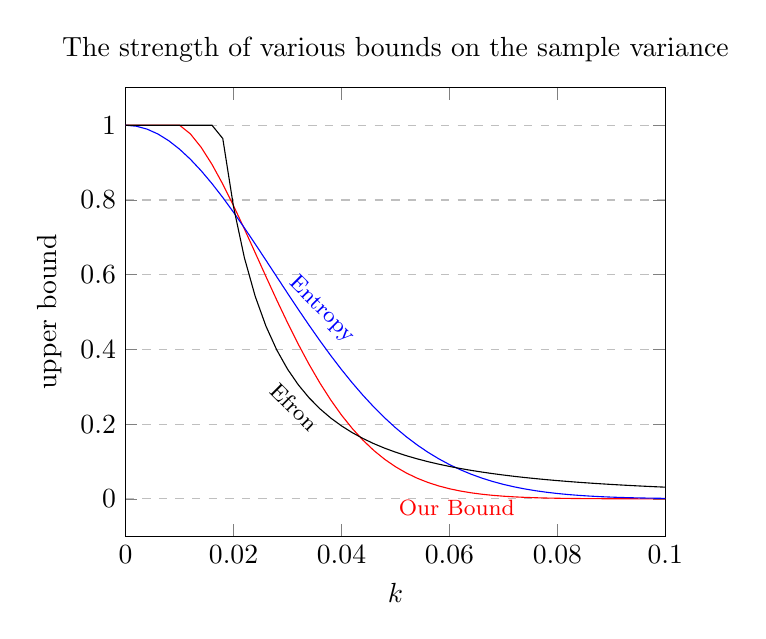
\begin{tikzpicture}
		\begin{axis}[
			title={The strength of various bounds on the sample variance},
			xlabel={$k$},
			ylabel={upper bound},
			xmin=0, xmax=0.1,
			%ymin=0.001, ymax=0.05,
			%ymode=log,
			%xtick={0,0.05,0.1,0.15,0.2,0.25},
			%ytick={0,20,40,60,80,100},
			%yticklabel=$\pgfmathprintnumber{\tick}\%$,
			legend pos=south west,
			ymajorgrids=true,
			grid style=dashed,
			xticklabel style={/pgf/number format/fixed}
		]
		\addplot[color={rgb:red,1;green,0;yellow,0}] coordinates {
(0.000000, 1.000000)(0.002000, 1.000000)(0.004000, 1.000000)(0.006000, 1.000000)(0.008000, 1.000000)(0.010000, 1.000000)(0.012000, 0.976796)(0.014000, 0.940761)(0.016000, 0.895277)(0.018000, 0.842473)(0.020000, 0.784293)(0.022000, 0.722562)(0.024000, 0.658973)(0.026000, 0.595056)(0.028000, 0.532153)(0.030000, 0.471397)(0.032000, 0.413695)(0.034000, 0.359740)(0.036000, 0.310013)(0.038000, 0.264798)(0.040000, 0.224211)(0.042000, 0.188221)(0.044000, 0.156675)(0.046000, 0.129339)(0.048000, 0.105899)(0.050000, 0.086012)(0.052000, 0.069309)(0.054000, 0.055417)(0.056000, 0.043973)(0.058000, 0.034631)(0.060000, 0.027074)(0.062000, 0.021015)(0.064000, 0.016197)(0.066000, 0.012397)(0.068000, 0.009425)(0.070000, 0.007118)(0.072000, 0.005341)(0.074000, 0.003983)(0.076000, 0.002951)(0.078000, 0.002173)(0.080000, 0.001591)(0.082000, 0.001158)(0.084000, 0.000838)(0.086000, 0.000603)(0.088000, 0.000431)(0.090000, 0.000307)(0.092000, 0.000217)(0.094000, 0.000153)(0.096000, 0.000107)(0.098000, 0.000074)(0.100000, 0.000052)(0.102000, 0.000035)(0.104000, 0.000024)(0.106000, 0.000017)(0.108000, 0.000011)(0.110000, 0.000008)(0.112000, 0.000005)(0.114000, 0.000003)(0.116000, 0.000002)(0.118000, 0.000001)(0.120000, 0.000001)(0.122000, 0.000001)(0.124000, 0.000000)(0.126000, 0.000000)(0.128000, 0.000000)(0.130000, 0.000000)(0.132000, 0.000000)(0.134000, 0.000000)(0.136000, 0.000000)(0.138000, 0.000000)(0.140000, 0.000000)(0.142000, 0.000000)(0.144000, 0.000000)(0.146000, 0.000000)(0.148000, 0.000000)
        }node[pos=0.91](endofplotsquare){} ;
		\node [below,color={rgb:red,1;green,0;yellow,0}] at (endofplotsquare) {\footnotesize Our Bound};
		\addplot[color={rgb:red,0;blue,1;yellow,0}] coordinates {
(0, 1.0) (0.002, 0.997350183644) (0.004, 0.989442789364) (0.006, 0.976402871073) (0.008, 0.958435191453) (0.01, 0.935818872672) (0.012, 0.908900183468) (0.014, 0.87808372306) (0.016, 0.843822315395) (0.018, 0.806605966074) (0.02, 0.766950257277) (0.022, 0.725384562782) (0.024, 0.682440455785) (0.026, 0.638640657998) (0.028, 0.594488841053) (0.03, 0.550460543126) (0.032, 0.506995407644) (0.034, 0.464490890034) (0.036, 0.423297515852) (0.038, 0.383715712221) (0.04, 0.345994177074) (0.042, 0.310329699467) (0.044, 0.276868301049) (0.046, 0.245707534782) (0.048, 0.216899752983) (0.05, 0.19045614263) (0.052, 0.166351321354) (0.054, 0.144528291741) (0.056, 0.124903563263) (0.058, 0.107372268989) (0.06, 0.0918131266269) (0.062, 0.0780931188187) (0.064, 0.0660717944596) (0.066, 0.0556051197572) (0.068, 0.0465488335613) (0.07, 0.0387612852497) (0.072, 0.0321057544037) (0.074, 0.0264522691726) (0.076, 0.0216789543788) (0.078, 0.0176729510065) (0.08, 0.0143309558975) (0.082, 0.0115594345264) (0.084, 0.00927456102917) (0.086, 0.00740193865015) (0.088, 0.00587615094073) (0.09, 0.00464018983902) (0.092, 0.00364480164518) (0.094, 0.0028477862716) (0.096, 0.00221327933787) (0.098, 0.0017110409802) (0.1, 0.0013157698685) (0.102, 0.00100645602988) (0.104, 0.00076578176314) (0.106, 0.000579576245108) (0.108, 0.000436326387277) (0.11, 0.000326744076771) (0.112, 0.00024338808442) (0.114, 0.000180337583441) (0.116, 0.000132913325077) (0.118, 9.74419898103e-05) (0.12, 7.10590028484e-05) (0.122, 5.15451037129e-05) (0.124, 3.71921316689e-05) (0.126, 2.6693779426e-05) (0.128, 1.90574332941e-05) (0.13, 1.35336235817e-05) (0.132, 9.56002706345e-06) (0.134, 6.71737346447e-06) (0.136, 4.6949958307e-06) (0.138, 3.26412116474e-06) (0.14, 2.25731764273e-06) (0.142, 1.55279607415e-06) (0.144, 1.06250630718e-06) (0.146, 7.23175913889e-07) (0.148, 4.89611639113e-07)
        }node[pos=0.5](endofplotsquare){} ;
		\node [above,color={rgb:red,0;blue,1;yellow,0}, rotate=-45] at (endofplotsquare) {\footnotesize Entropy};
		\addplot[black] coordinates {
(0, 1) (0.002, 1.0) (0.004, 1.0) (0.006, 1.0) (0.008, 1.0) (0.01, 1.0) (0.012, 1.0) (0.014, 1.0) (0.016, 1.0) (0.018, 0.96450617284) (0.02, 0.78125) (0.022, 0.645661157025) (0.024, 0.542534722222) (0.026, 0.462278106509) (0.028, 0.398596938776) (0.03, 0.347222222222) (0.032, 0.30517578125) (0.034, 0.270328719723) (0.036, 0.24112654321) (0.038, 0.216412742382) (0.04, 0.1953125) (0.042, 0.177154195011) (0.044, 0.161415289256) (0.046, 0.147684310019) (0.048, 0.135633680556) (0.05, 0.125) (0.052, 0.115569526627) (0.054, 0.107167352538) (0.056, 0.0996492346939) (0.058, 0.0928953626635) (0.06, 0.0868055555556) (0.062, 0.0812955254943) (0.064, 0.0762939453125) (0.066, 0.0717401285583) (0.068, 0.0675821799308) (0.07, 0.0637755102041) (0.072, 0.0602816358025) (0.074, 0.0570672023375) (0.076, 0.0541031855956) (0.078, 0.0513642340565) (0.08, 0.048828125) (0.082, 0.0464753123141) (0.084, 0.0442885487528) (0.086, 0.0422525689562) (0.088, 0.040353822314) (0.09, 0.0385802469136) (0.092, 0.0369210775047) (0.094, 0.0353666817565) (0.096, 0.0339084201389) (0.098, 0.0325385256143) (0.1, 0.03125) (0.102, 0.0300365244137) (0.104, 0.0288923816568) (0.106, 0.0278123887504) (0.108, 0.0267918381344) (0.11, 0.025826446281) (0.112, 0.0249123086735) (0.114, 0.0240458602647) (0.116, 0.0232238406659) (0.118, 0.02244326343) (0.12, 0.0217013888889) (0.122, 0.0209957000806) (0.124, 0.0203238813736) (0.126, 0.0196837994457) (0.128, 0.0190734863281) (0.13, 0.0184911242604) (0.132, 0.0179350321396) (0.134, 0.0174036533749) (0.136, 0.0168955449827) (0.138, 0.0164093677799) (0.14, 0.015943877551) (0.142, 0.0154979170799) (0.144, 0.0150704089506) (0.146, 0.0146603490336) (0.148, 0.0142668005844)
        }node[pos=0.7](endofplotsquare){} ;
		\node [below,black, rotate=-45] at (endofplotsquare) {\footnotesize Efron};
		
		\end{axis}
		\end{tikzpicture}
		%\vspace{-18pt}
		\caption[Comparrison of bound strengths on the variance]{The upper bound on $ \p(\sigma^2-\hat{\sigma}^2\ge k) $ for various $k$, at $\sigma^2=0.1$ for $D=1, n=200$ using the Entropy method (Equation \ref{eq:fe}), the Efron-Stein method (Equation \ref{eq:efron_stein_eq}), and our method (via Theorem \ref{variance2})}
		\label{fig:variance_graph1}
    \end{figure}
